%%%%%%%%%%%%%%%%%%%%%%%%%%%%%%%%%
% 6CCS3PRJ Final Year Individual Project Report -- Appendices volume
%
% This file produces the appendices-only PDF that is submitted alongside
% report.pdf. The preamble mirrors report.tex so the typesetting matches.
% Cross-references to labels defined in the main report are resolved via
% the xr package (\externaldocument{report}); for those references to
% appear correctly the main report.aux must already exist when this file
% is compiled. The recommended build order is therefore:
%   pdflatex report.tex     (twice, with bibtex in between)
%   pdflatex report-appendices.tex   (twice)
%%%%%%%%%%%%%%%%%%%%%%%%%%%%%%%%%
\documentclass[11pt]{informatics-report}
\usepackage{color}
\usepackage[square,sort,comma,numbers]{natbib}
\usepackage{parskip}
\usepackage{float}
\usepackage{adjustbox}
\usepackage{array}
\newcolumntype{P}[1]{>{\raggedright\arraybackslash}p{#1}}
\usepackage{longtable}
\usepackage{enumitem}
\usepackage{needspace}
\usepackage{graphicx}
\usepackage[implicit=false]{hyperref}
\usepackage{pdfpages}
\usepackage{soul}
\usepackage{xcolor}
\definecolor{linkhl}{RGB}{210, 230, 255}

\setkeys{Gin}{interpolate=false}
\usepackage{listings}
\lstset{
  language=[ISO]C++,
  basicstyle=\small\ttfamily,
  keywordstyle=\bfseries,
  commentstyle=\itshape,
  breaklines=true,
  frame=single,
  numbers=none,
  xleftmargin=2em,
  framexleftmargin=1.5em,
  aboveskip=1em,
  belowskip=1em,
  columns=flexible
}
\usepackage{tabularx}
\usepackage{xltabular}
\usepackage{subcaption}
\usepackage{float}

%% Resolve cross-references to the main report (sections, figures, chapters).
%% Compile report.tex first so report.aux is available.
\usepackage{xr}
\externaldocument{report}

%%%%%%%%%%%%%%%%%%%%%%%%%%%%%%%%%
% Front Matter
%%%%%%%%%%%%%%%%%%%%%%%%%%%%%%%%%
\title{6CCS3PRJ \\\vspace{0.2cm}Designing for Consent Revocation in Online Platforms: WhatsApp Photo Sharing}
\author{Mert Ayranci}
\studentID{21175534}
\supervisor{Kovila Coopamootoo}
\date{\today}

\begin{document}

%% Custom cover page for the appendices volume. We deliberately do not call
%% \createFrontMatter (defined in informatics-report.cls) because that
%% command emits the abstract and originality avowal of the main report,
%% which are inappropriate for an appendices-only file.
\makeatletter
\thispagestyle{empty}
\begin{center}
  \begin{flushright}
    
\includegraphics[scale=0.4]{FrontMatter/logo.png}\\*
  \end{flushright}
  \vspace*{2.2in}
  {\huge \bfseries \@title\par}
  \vspace*{0.4in}
  {\Large Final Project Report --- Appendices\par}
  \vspace*{1.2in}
  {\large
    Author: \@author\\*
    Supervisor: \@supervisor\\*
    Student ID: \@studentID\\*
    \vspace*{0.2in}
    \@date\par}
\end{center}
\makeatother
\clearpage

\thispagestyle{empty}
\noindent
\textbf{About this document.} This file contains the appendices that accompany the main project report (\textit{report.pdf}). It is submitted as a separate PDF in line with the university's submission instructions. Cross-references of the form ``Section~X'' or ``Chapter~X'' refer to the main report unless stated otherwise.
\clearpage

\onehalfspacing
\setcounter{tocdepth}{1}
\renewcommand{\contentsname}{Contents of appendices}
\tableofcontents
\doublespacing

%%%%%%%%%%%%%%%%%%%%%%%%%%%%%%%%%
% Appendices
%%%%%%%%%%%%%%%%%%%%%%%%%%%%%%%%%
\appendix
\chapter{Thematic Analysis Materials}
\label{app:codebook}

This appendix reproduces the reflexive thematic analysis workbook as exported from the project Miro board.

\newpage
\section{Interview extracts board (raw)}
\label{app:thematic-quotes-raw}

\noindent
First page of the full colour-coded transcript extract board.

\begin{center}
  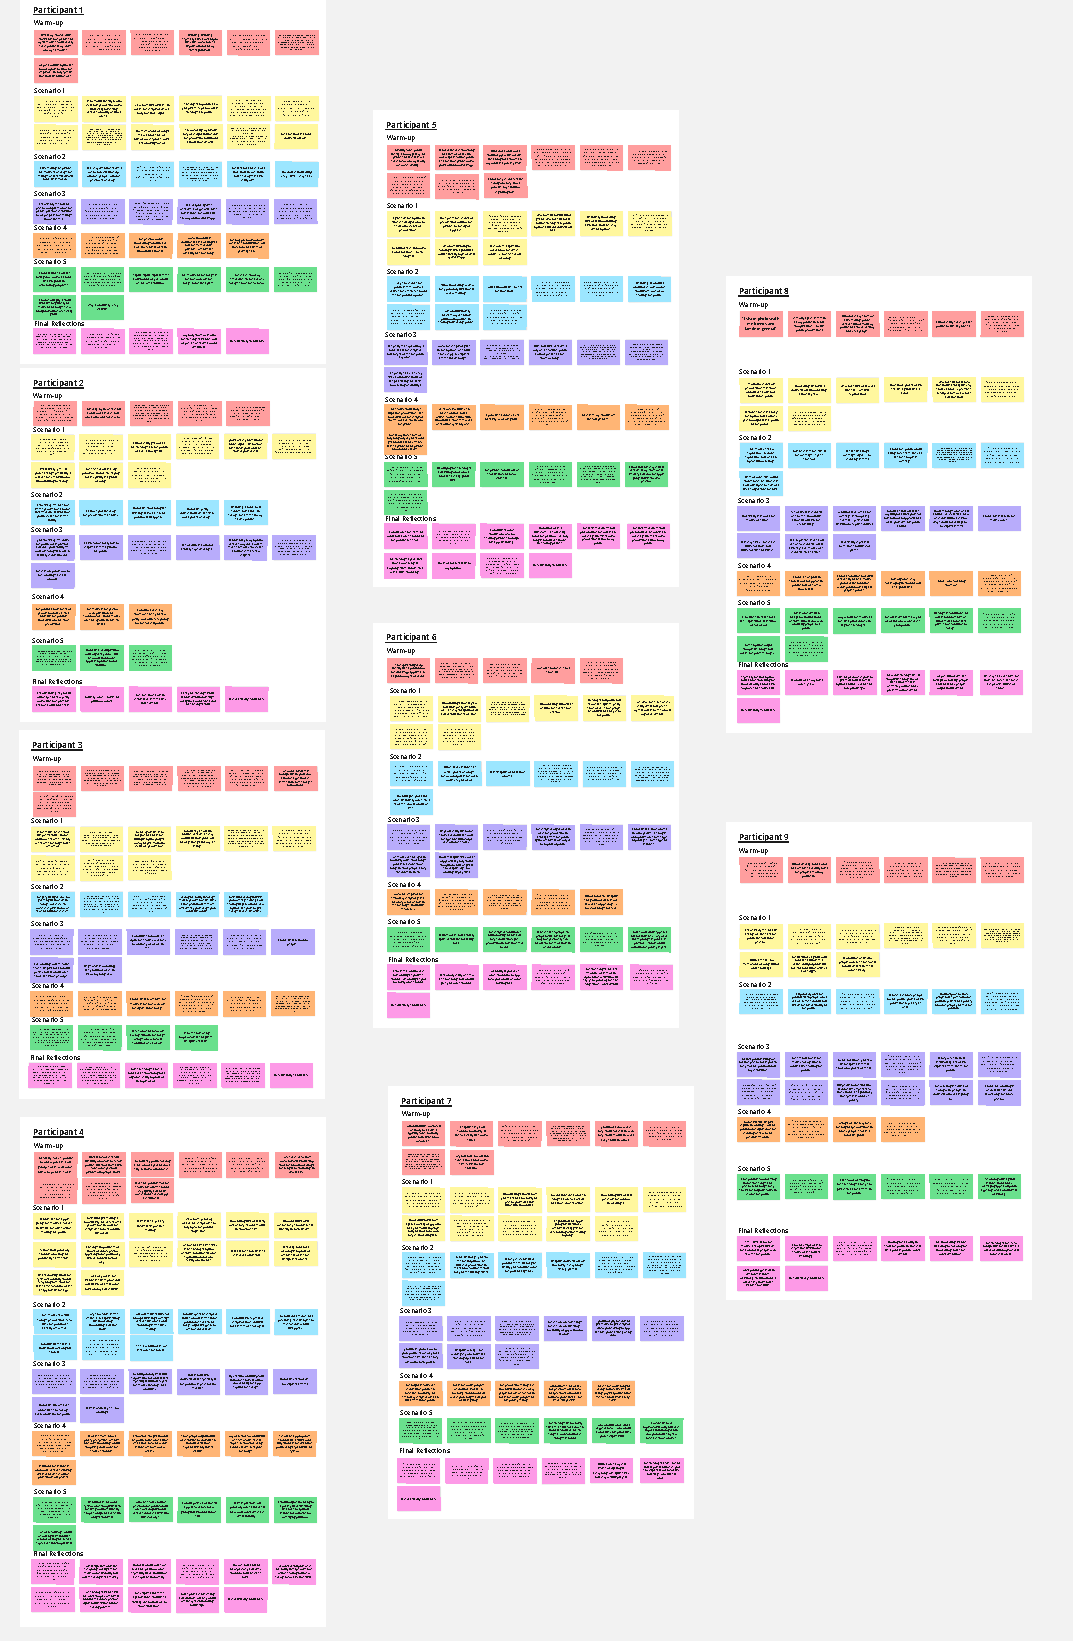
\includegraphics[page=1,width=0.75\textwidth]{appendix-materials/thematic-analysis/interview-extracts-raw-board.pdf}
\end{center}

\newpage
\section{Inductive codebook (initial iteration)}
\label{app:thematic-codebook-initial}

\noindent
First page of the initial 56-code codebook produced through close reading of the interview transcripts.

\begin{center}
  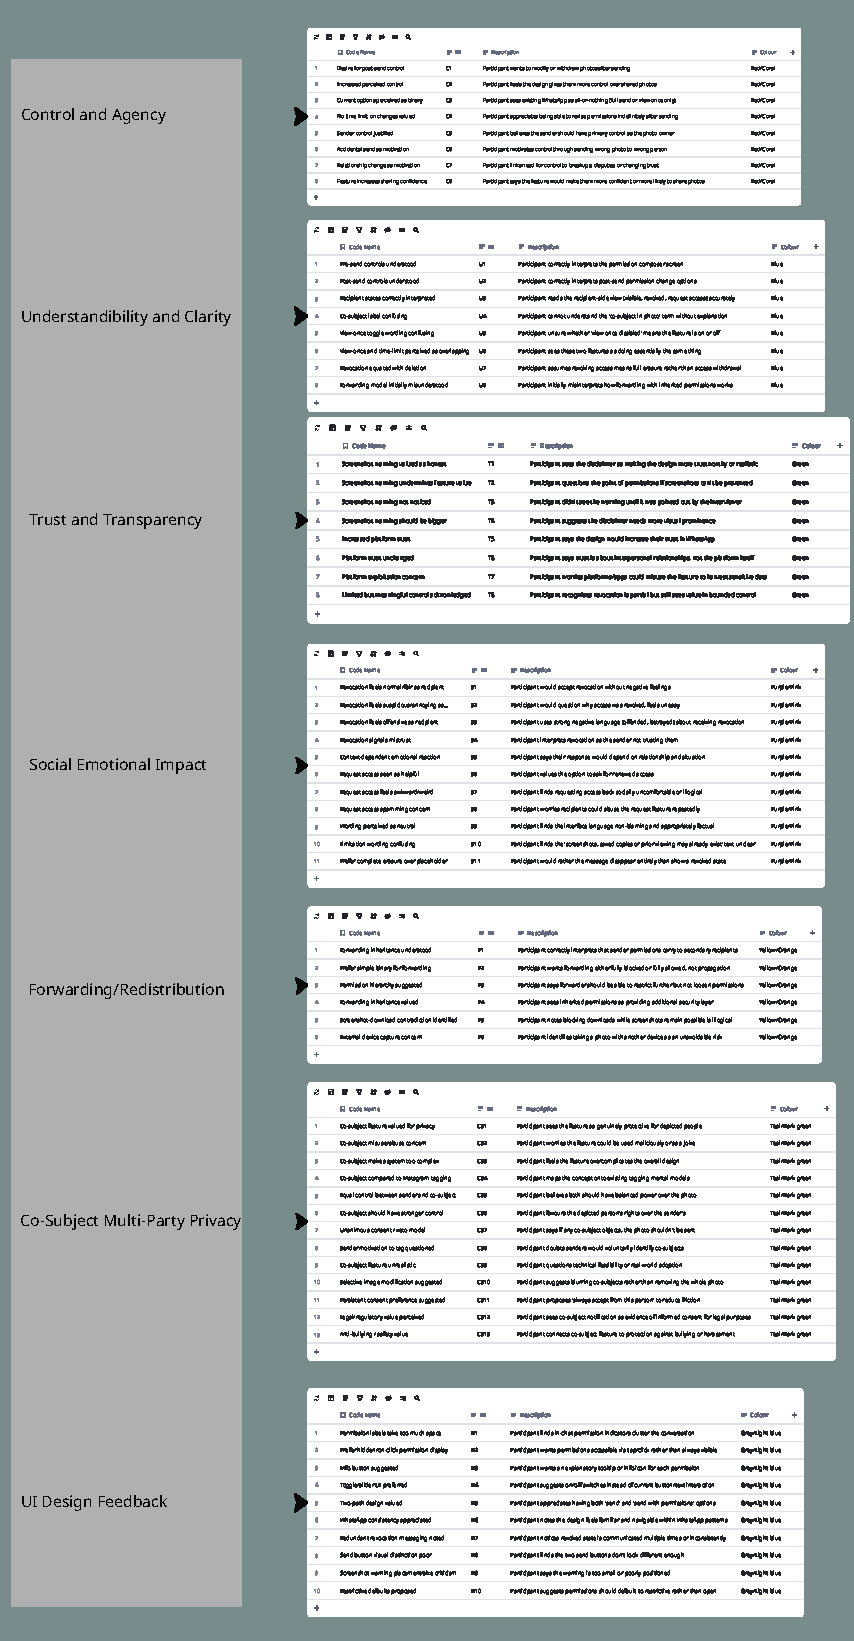
\includegraphics[page=1,width=0.75\textwidth]{appendix-materials/thematic-analysis/inductive-codebook-initial.pdf}
\end{center}


\section{Interview extracts (refined subset)}
\label{app:thematic-quotes-refined}

\noindent
First page of the refined extract set used for focused coding.

\begin{center}
  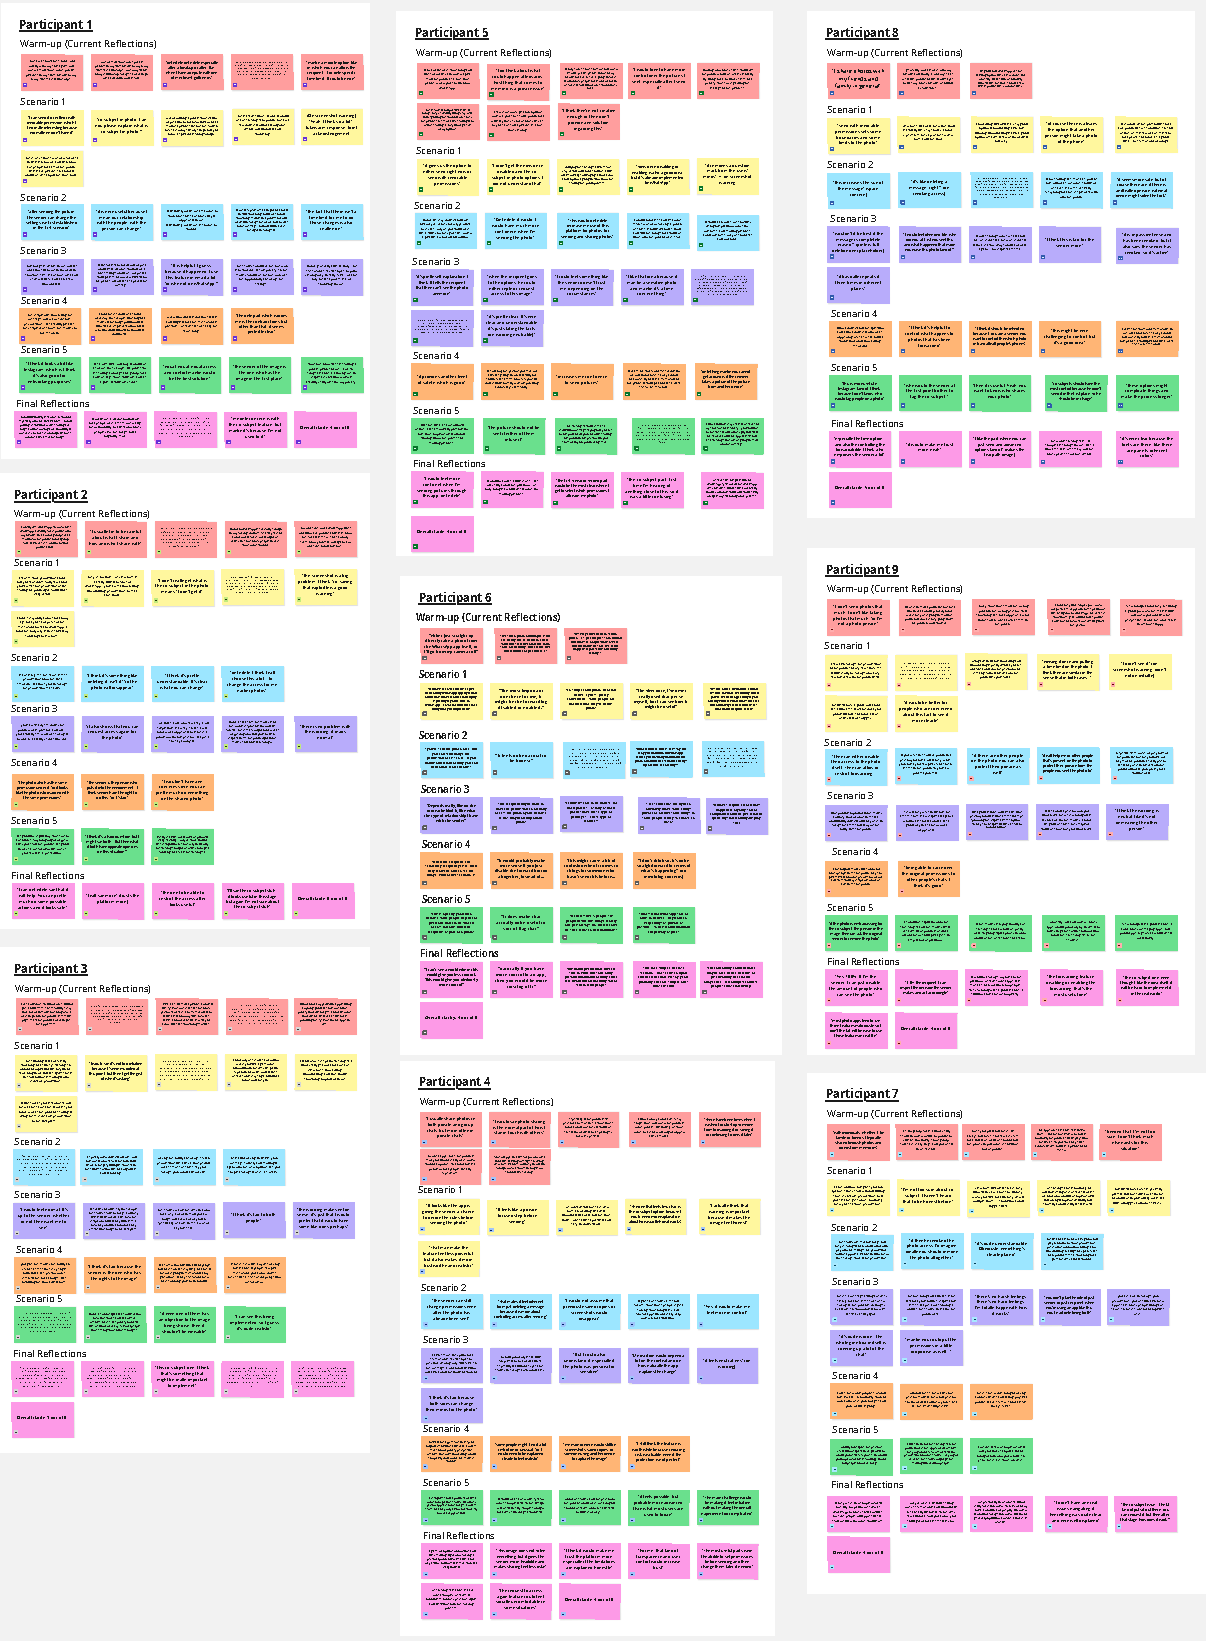
\includegraphics[page=1,width=\textwidth]{appendix-materials/thematic-analysis/interview-extracts-refined.pdf}
\end{center}

\newpage
\section{Working codebook (simplified)}
\label{app:thematic-codebook-working}

\noindent
First page of the simplified 20-code working codebook used for cross-case tagging.

\begin{center}
  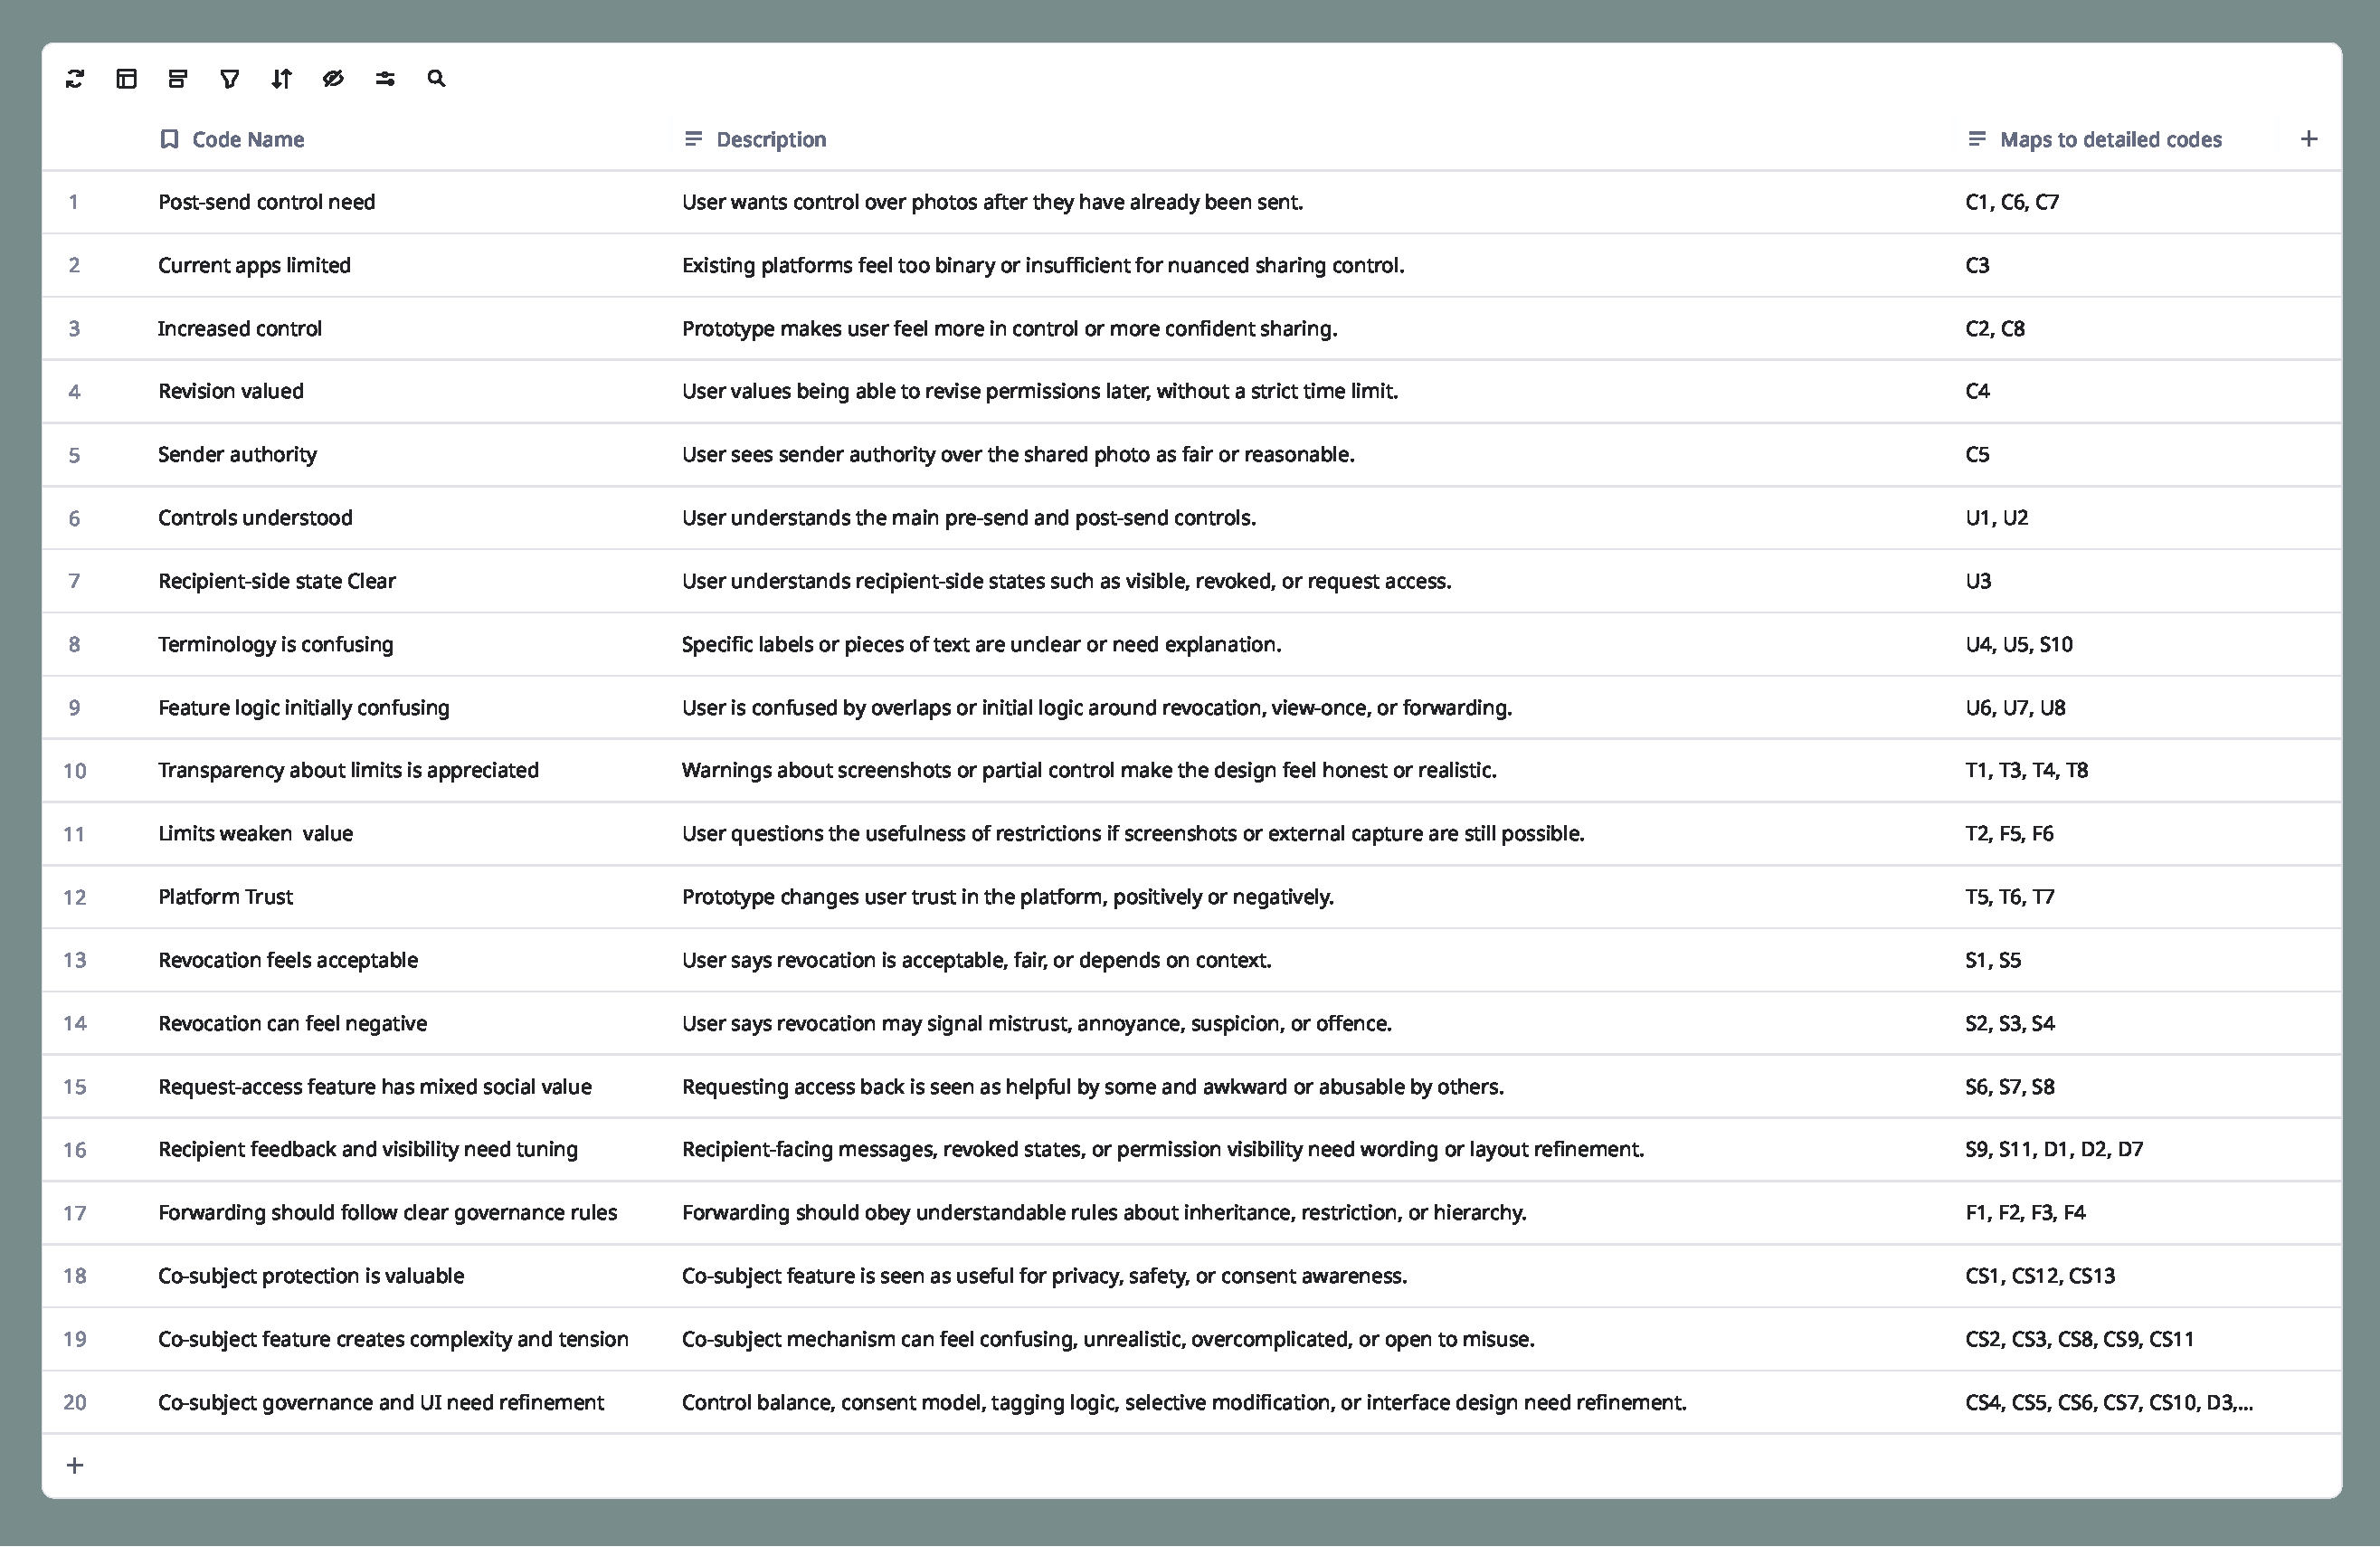
\includegraphics[page=1,width=\textwidth,height=0.88\textheight,keepaspectratio]{appendix-materials/thematic-analysis/working-codebook-simplified.pdf}
\end{center}

\newpage
\section{Quote-to-code coding sheet}
\label{app:thematic-coding-sheet}

\noindent
First page of the quote-to-code mapping sheet.

\begin{center}
  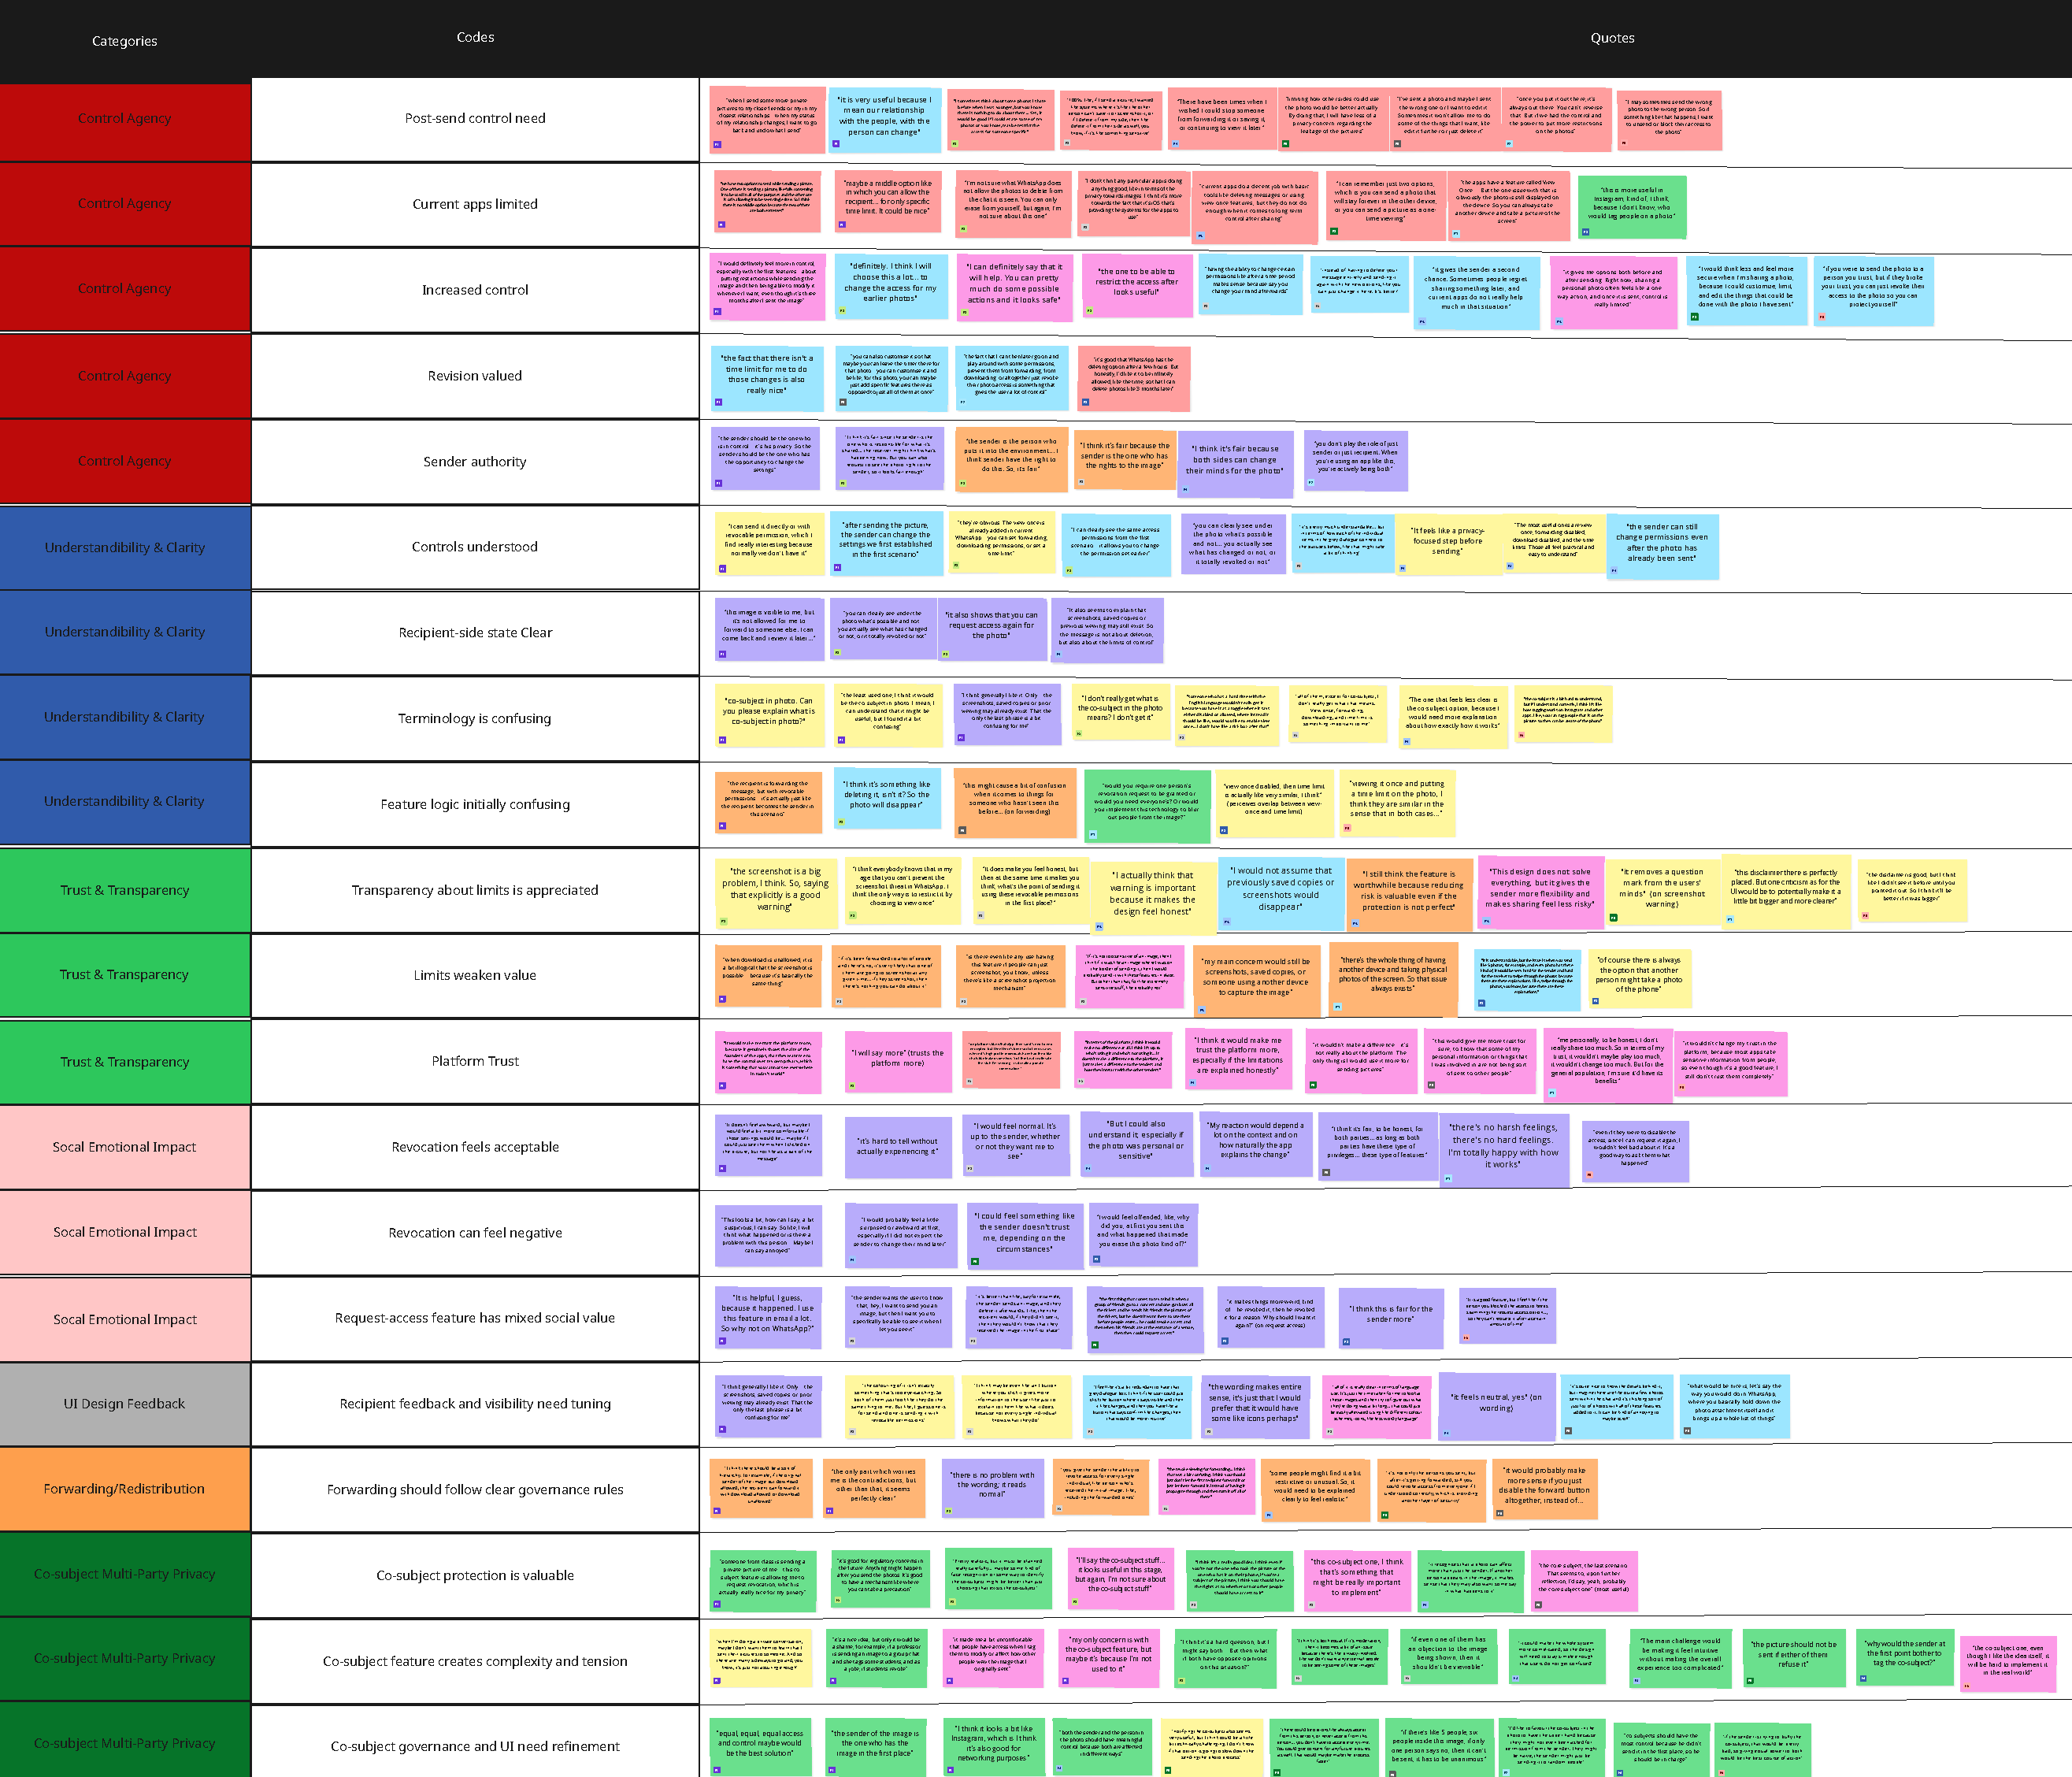
\includegraphics[page=1,width=\textwidth,height=0.88\textheight,keepaspectratio]{appendix-materials/thematic-analysis/quote-to-code-coding-sheet.pdf}
\end{center}

\newpage
\section{Final themes table}
\label{app:thematic-themes-table}

\noindent
First page of the consolidated themes table (definitions, codes, and example quotations).

\begin{center}
  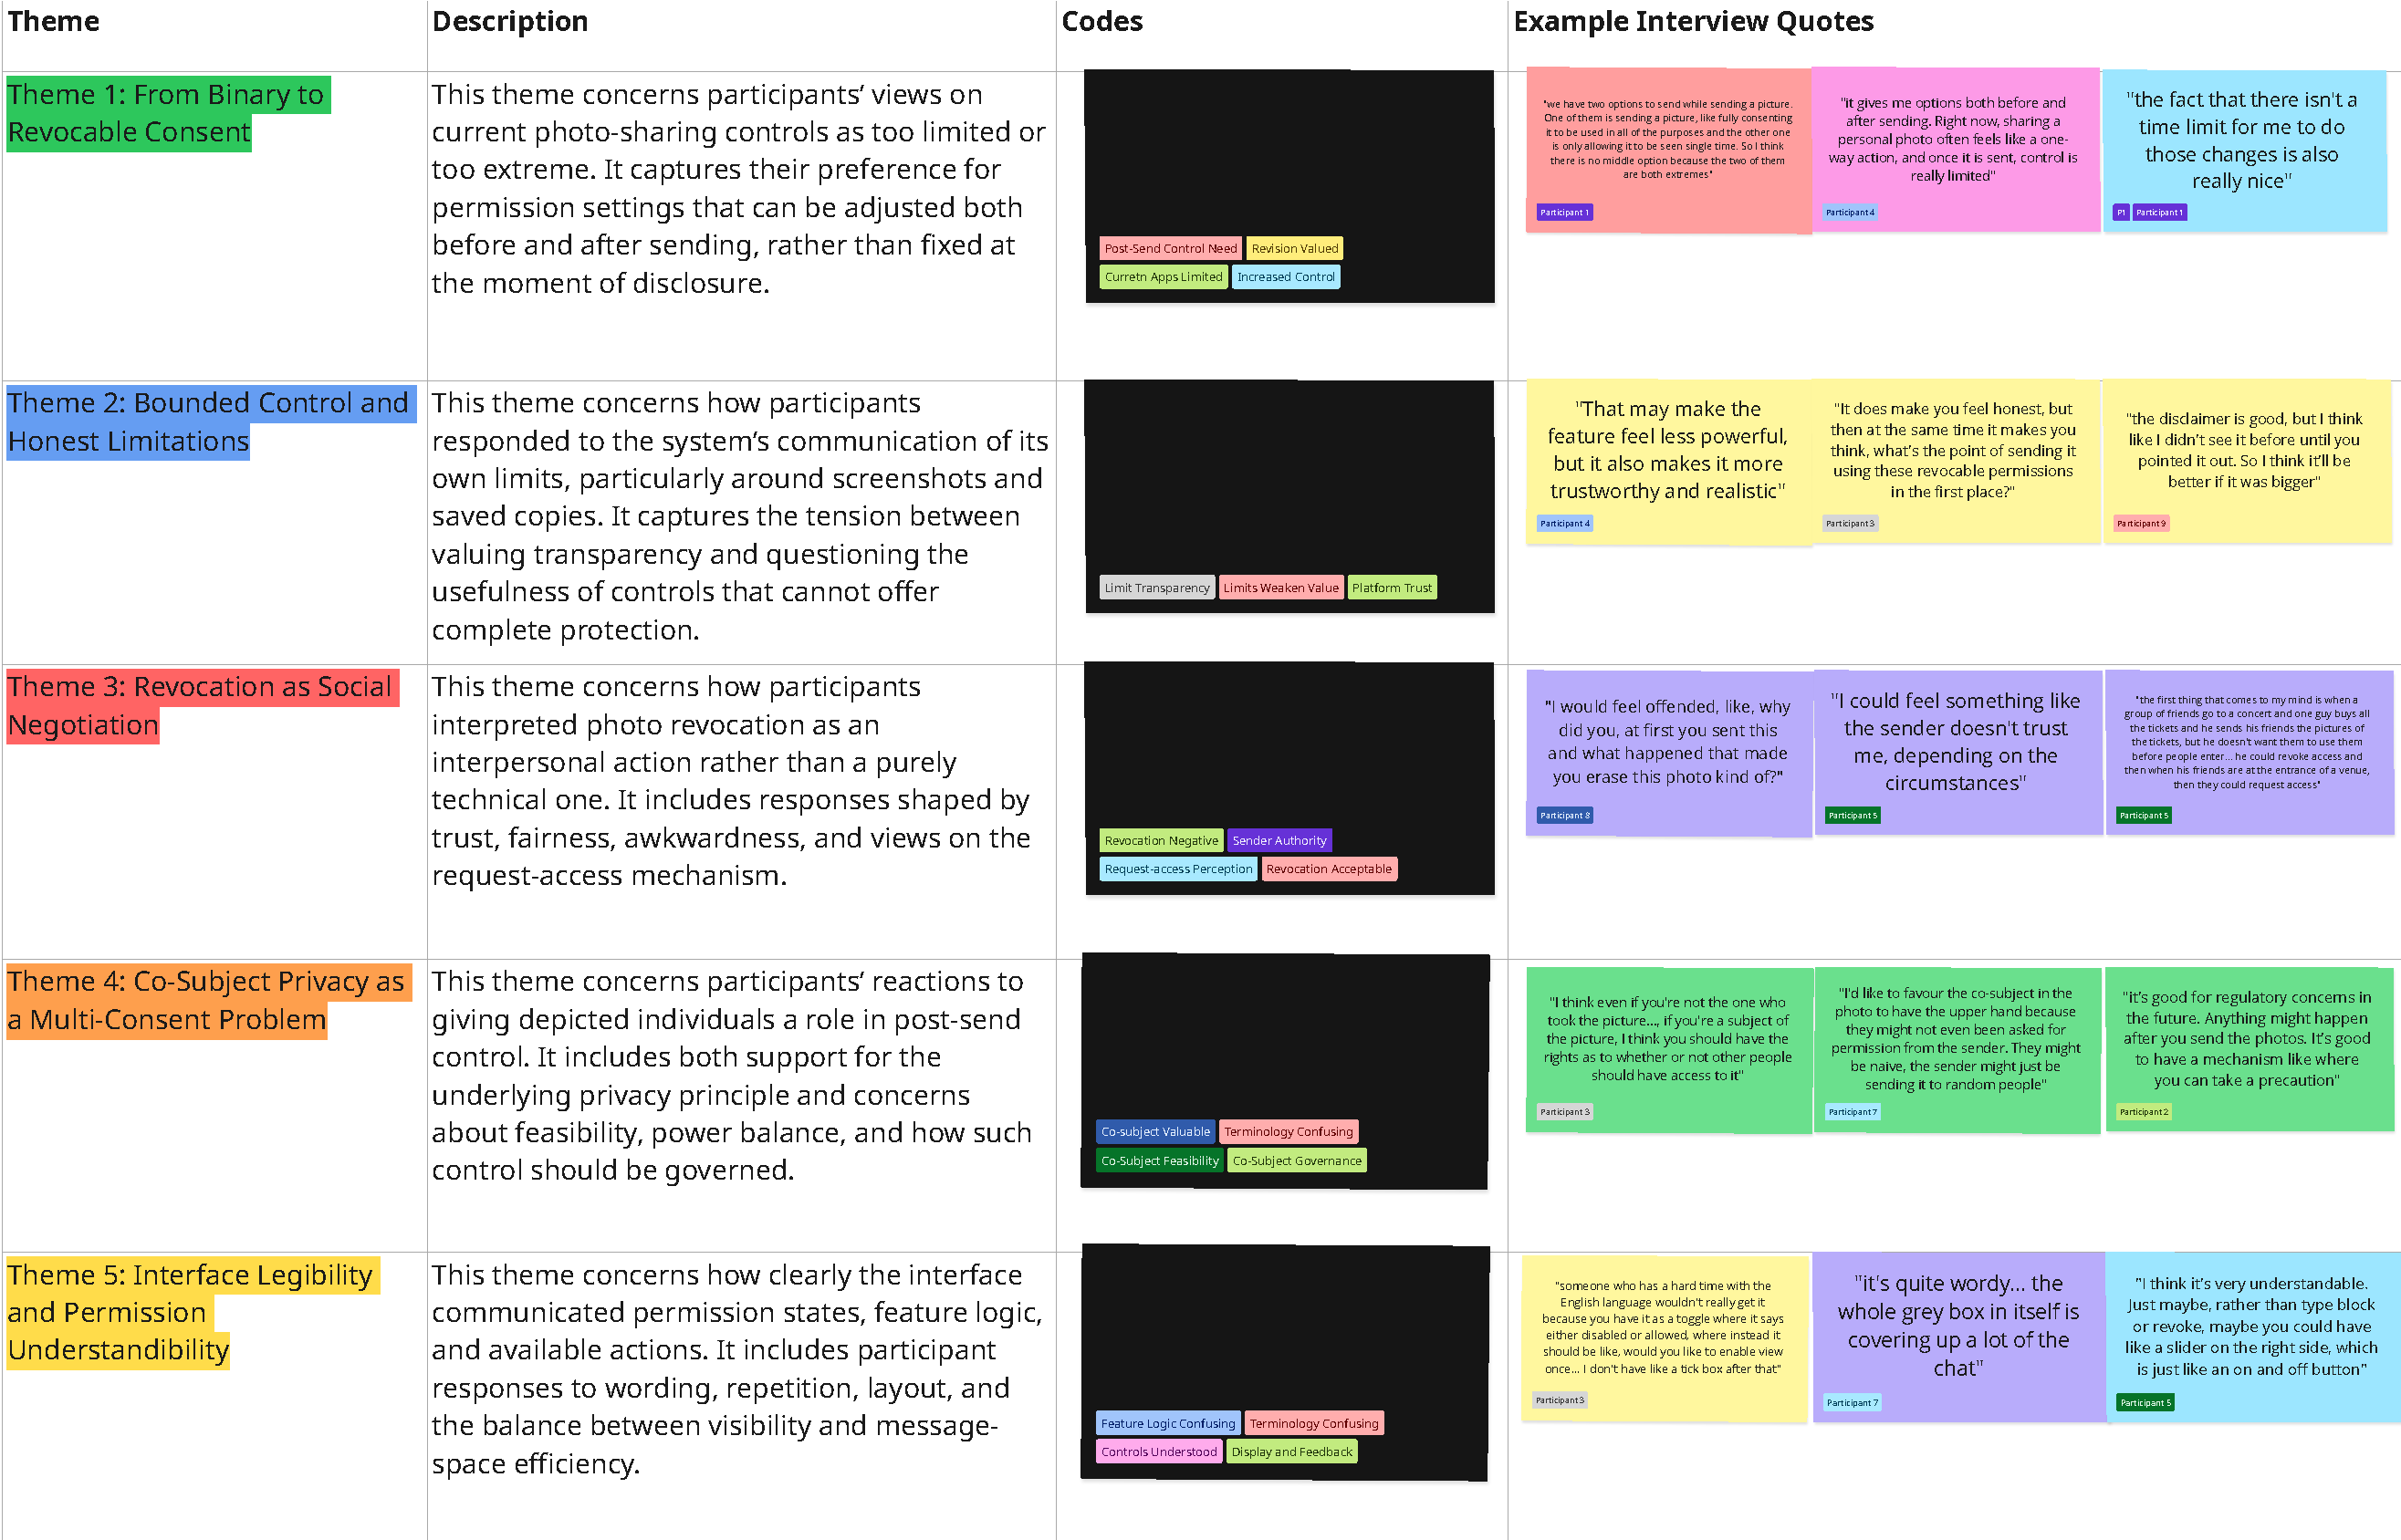
\includegraphics[page=1,width=\textwidth,height=0.88\textheight,keepaspectratio]{appendix-materials/thematic-analysis/final-themes-table.pdf}
\end{center}








\chapter{Interview Guide}
\label{app:interview-guide}

This appendix records the scenario-based moderator script used in the evaluation interviews. The wording follows the version spoken in sessions (including the consent statement and scenario prompts). Each numbered question lists the \textbf{linked research questions} (Main~RQ and RQ1--RQ5) taken from the analysis mapping used alongside the guide: RQ1 addresses current platform limitations; RQ2 expectations and post-sharing concerns; RQ3 clarity of the interface and permission model; RQ4 fairness and social implications; RQ5 trust, safety, control, and realism of revocation. The main research question is stated in Chapter~1.

\section*{Research question key}
\begin{description}[style=nextline,leftmargin=0.8cm]
  \item[Main~RQ] Overall contribution of the proposed design.
  \item[RQ1] Limitations of current platforms for controlling shared photos.
  \item[RQ2] User expectations, practices, and concerns about post-sharing control.
  \item[RQ3] Clarity and understandability of the interface and permission model.
  \item[RQ4] Social implications for stakeholders.
  \item[RQ5] Trust, safety, perceived control, and realism of revocation.
\end{description}

\section{Section 0: Mandatory consent statement}
\textit{Say verbatim:}

\begin{quote}\small\sloppy
``Before we begin, I'd like to confirm your consent to participate in this interview. This interview is part of my research on how messaging platforms might support consent revocation for shared photos. The purpose of this interview is to understand your views and reactions to a design concept. During the interview, I will show you example screens from a prototype. I am not testing you --- I am testing the design. There are no right or wrong answers, and honest reactions are very helpful. Some questions are about privacy, control, and what happens to photos after they are shared. You can skip any question or stop the interview at any time. With your permission, I would like to audio-record this interview so I can analyse the responses later. The recording will only be used for this project, and your responses will be anonymised. You can choose to stop the recording or withdraw from the interview at any time. If you're happy to proceed, could you please state your full name and age, and confirm that you agree to be interviewed and recorded?''
\end{quote}

\section{Section 1: Warm-up and current photo-sharing behaviour}


\begin{enumerate}
  \item \textbf{Can you tell me a bit about how you usually share photos on apps like WhatsApp?}\\
  \textit{Linked:} RQ2.\\
  \textit{Probes optional:} private vs group chats; casual vs personal photos; frequency.

  \item \textbf{When you send a photo to someone, do you usually think about what might happen to it afterwards? If yes, what kinds of concerns or challenges come to mind?}\\
  \textit{Linked:} RQ2.\\
  \textit{Probes optional:} saving, forwarding, screenshots, long-term retention; active vs incidental thought.

  \item \textbf{Have you ever wanted more control over a photo after you had already sent it?}\\
  \textit{Linked:} RQ1; RQ2.\\
  \textit{Probes optional:} type of control wished for; whether the app helped.

  \item \textbf{What do you think current apps do well or badly when it comes to controlling shared photos?}\\
  \textit{Linked:} RQ1.
\end{enumerate}


\section{Section 2: Scenario 1 --- Before sending a photo}
\textit{Show:} photo composer / permission setup (view once, forwarding, download, co-subject, time limit; note on screenshots and saves).


\begin{enumerate}[resume]
  \item \textbf{What do you think is happening on this screen?}\\
  \textit{Linked:} RQ3.\\
  \textit{Probes optional:} purpose of controls; what the sender decides.

  \item \textbf{What do you think each of these settings means?}\\
  \textit{Linked:} RQ3.\\
  \textit{Probes optional:} view once; forwarding disabled; download disabled; time limit; co-subject in photo.

  \item \textbf{Which of these options feel useful to you, and which feel unnecessary or unclear?}\\
  \textit{Linked:} RQ2; RQ3.\\
  \textit{Probes optional:} realistic pre-send use; effort; missing options.

  \item \textbf{There is also a warning here saying that screenshots and saves cannot be undone. How do you feel about that?}\\
  \textit{Linked:} RQ3; RQ5.\\
  \textit{Probes optional:} honesty vs usefulness; whether the warning is wanted.
\end{enumerate}

\textit{Moderator note:} Only explain controls if the participant is completely stuck; prior interpretation is the primary data.

\section{Section 3: Scenario 2 --- Changing permissions after sending}
\textit{Show:} sent photo with photo menu (revoke/restore, forwarding, download, time limit).


\begin{enumerate}[resume]
  \item \textbf{Looking at this screen, what do you think the sender is able to do now?}\\
  \textit{Linked:} RQ3.\\
  \textit{Probes optional:} what is changeable after send; comparison to deleting a message; revoke vs permission change.

  \item \textbf{What would you expect to happen if the sender revokes access here?}\\
  \textit{Linked:} RQ3; RQ5.\\
  \textit{Probes optional:} visibility; recipient notification; offline copies; if already seen.

  \item \textbf{How understandable does this post-send control feel to you?}\\
  \textit{Linked:} RQ3.\\
  \textit{Probes optional:} clarity of change; menu affordances; discoverability.

  \item \textbf{Would this kind of feature make you feel more in control after sending a photo? Why or why not?}\\
  \textit{Linked:} RQ5.\\
  \textit{Probes optional:} trust; anxiety; realistic use.
\end{enumerate}

\textit{Moderator note:} Keep focus on clarity, expectations, realism, and perceived control rather than implementation detail.

\section{Section 4: Scenario 3 --- Recipient view, request access, and fairness}
\textit{Show:} recipient-side revoked placeholder (screenshots / prior viewing note).


\begin{enumerate}[resume]
  \item \textbf{What do you think this screen is telling the recipient?}\\
  \textit{Linked:} RQ3; RQ4.\\
  \textit{Probes optional:} clarity of change; sufficiency of explanation.

  \item \textbf{How would you feel if you were the recipient in this situation?}\\
  \textit{Linked:} RQ4; RQ5.\\
  \textit{Probes optional:} reasonable vs awkward; fairness tone.

  \item \textbf{What do you think about the idea that the recipient can request access again?}\\
  \textit{Linked:} RQ4.\\
  \textit{Probes optional:} comfort as sender or recipient; balance.

  \item \textbf{Does this feel fair to both people, or more fair to one side than the other?}\\
  \textit{Linked:} RQ4.\\
  \textit{Probes optional:} sender power; explanation; objection rights.

  \item \textbf{What do you think about the wording used here?}\\
  \textit{Linked:} RQ4.\\
  \textit{Probes optional:} neutrality vs blame.
\end{enumerate}

\textit{Moderator note:} Do not defend the revoked state; negative reactions are informative.

\section{Section 5: Scenario 4 --- Forwarding and residual concerns}
\textit{Show:} forwarding behaviour and secondary recipient where relevant; request-access flow and sender accept/reject if shown.


\begin{enumerate}[resume]
  \item \textbf{What do you think this forwarding feature is trying to do?}\\
  \textit{Linked:} RQ3.\\
  \textit{Probes optional:} blocked vs allowed forwarding; sender rules after forward.

  \item \textbf{How do you feel about the idea that the sender's rules continue even after the photo is forwarded?}\\
  \textit{Linked:} RQ3; RQ5.\\
  \textit{Probes optional:} usefulness; realism; over-control.

  \item \textbf{Even with these features, what concerns would still remain for you?}\\
  \textit{Linked:} RQ1; RQ2; RQ5.\\
  \textit{Probes optional:} screenshots; prior downloads; residual value of imperfect control.
\end{enumerate}

\section{Section 6: Scenario 5 --- Co-subject request for revocation}
\textit{Show:} co-subject notification and request flow; sender accept/reject.


\begin{enumerate}[resume]
  \item \textbf{What do you think about that idea?}\\
  \textit{Linked:} RQ4; RQ5.\\
  \textit{Probes optional:} fairness; invasiveness; complexity.

  \item \textbf{For this kind of scenario where the photo includes the sender and other co-subjects, who do you think should have the strongest control in that situation: the sender, the person in the photo, both equally, or someone else?}\\
  \textit{Linked:} RQ4.

  \item \textbf{How realistic does this feel in a real messaging app?}\\
  \textit{Linked:} RQ5.
\end{enumerate}

\textit{Moderator note:} Use only if time allows or if co-subject control is a session focus.

\section{Section 7: Wrap-up and final reflections}


\begin{enumerate}[resume]
  \setcounter{enumi}{24}
  \item \textbf{Would this make you feel more in control when sharing personal photos? Why or why not?}\\
  \textit{Linked:} RQ5.

  \item \textbf{Would it make you trust the platform more, less, or no differently?}\\
  \textit{Linked:} RQ5.

  \item \textbf{What part felt most clear or useful?}\\
  \textit{Linked:} RQ3; RQ5.

  \item \textbf{What part felt most confusing, unrealistic, or uncomfortable?}\\
  \textit{Linked:} RQ1; RQ3; RQ5.

  \item \textbf{From 1 to 5, how clear do you think everything feels?}\\
  \textit{Linked:} RQ3.
\end{enumerate}

\newpage
\section{Interview scenario slides (stimulus material)}
\label{app:interview-scenario-slides}

\noindent
This section reproduces the slide deck \emph{Consent Revocation Interview Scenarios}. The screenshots embedded in these slides were taken from the \textbf{first round} of the prototype implementation, before later visual or interaction refinements and they are preserved here to document the materials participants actually saw.

\begin{center}
  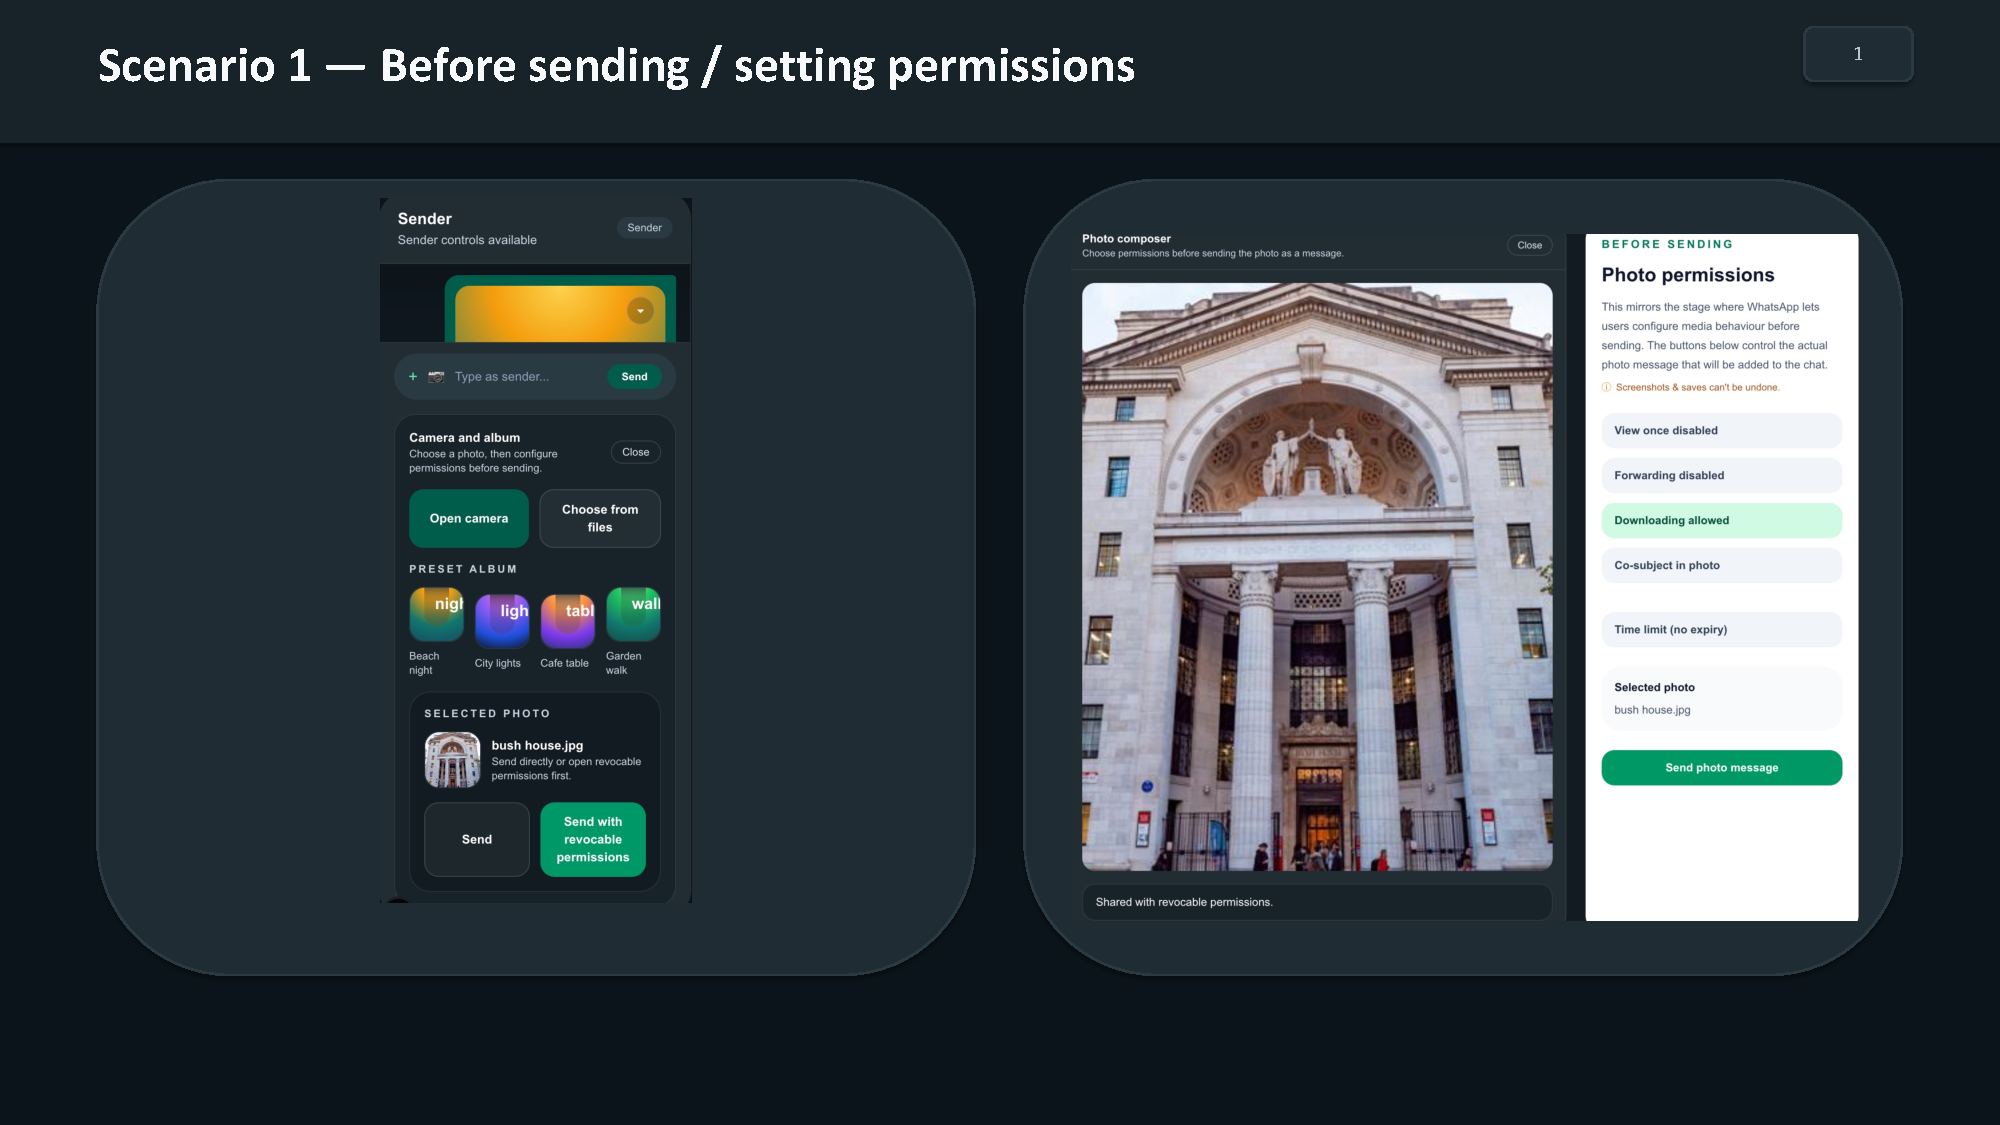
\includegraphics[page=1,width=\textwidth,height=0.88\textheight,keepaspectratio]{appendix-materials/interview/interview-scenario-slides.pdf}
\end{center}

\begin{center}
  \includegraphics[page=2,width=\textwidth,height=0.88\textheight,keepaspectratio]{appendix-materials/interview/interview-scenario-slides.pdf}
\end{center}
\newpage
\begin{center}
  \includegraphics[page=3,width=\textwidth,height=0.88\textheight,keepaspectratio]{appendix-materials/interview/interview-scenario-slides.pdf}
\end{center}

\begin{center}
  \includegraphics[page=4,width=\textwidth,height=0.88\textheight,keepaspectratio]{appendix-materials/interview/interview-scenario-slides.pdf}
\end{center}
\newpage
\begin{center}
  \includegraphics[page=5,width=\textwidth,height=0.88\textheight,keepaspectratio]{appendix-materials/interview/interview-scenario-slides.pdf}
\end{center}


\chapter{User Guide}
\label{app:user-guide}

\section{Purpose}
\label{sec:user-guide-purpose}

\noindent
 This appendix explains how to run the \textbf{Smart Photos} prototype on a local machine. Also a deployed version can be accessed at \url{https://smart-photos.vercel.app}.
A concise, illustrated tour of every major flow is already given in Section~\ref{sec:translation}. 

\section{Prerequisites}

\begin{itemize}
  \item \textbf{Node.js} version \textbf{20.x} (LTS recommended). The project uses TypeScript tooling aligned with Node~20; older major versions may fail to install or run dependencies.
  \item \textbf{npm} (bundled with Node.js). The instructions below use \texttt{npm}
\end{itemize}

\section{Install and run}

\begin{enumerate}
  \item Open a terminal and change into the prototype folder:
  \begin{verbatim}
cd photo-revocation-prototype
  \end{verbatim}
  \item Install dependencies:
  \begin{verbatim}
npm install
  \end{verbatim}
  \item Start the development server:
  \begin{verbatim}
npm run dev
  \end{verbatim}
  \item Open the default address printed in the terminal and make it full screen to have a better view. 
\end{enumerate}

\section{Optional: production build}

\noindent
To run an optimised build (closer to a deployed Next.js app, useful for a stable demo):

\begin{verbatim}
npm run build
npm run start
\end{verbatim}

\section{Feature checklist (where to see each behaviour)}


\begin{center}
\small
\begin{tabular}{@{}P{3.6cm}P{9.8cm}@{}}
\hline
\textbf{Feature} & \textbf{What to do in the running prototype} \\
\hline
Pre-send permissions and screenshot warning & From the sender handset, open the photo picker, choose one or more images, then use \emph{Send with revocable permissions}. \\
\hline
Post-send permission changes / revocation & On the sender handset, open the action menu on a sent photo message and use the post-send options (e.g.\ revoke access, forwarding, download, time limit). Expand the permission summary row under the bubble if needed. \\
\hline
Recipient view and revoked placeholder & Compare the recipient handset before and after sender-side revocation. Use recipient menu actions such as \emph{Forward}, \emph{Download}, or \emph{Request access} when the design allows them. \\
\hline
View-once consumption & On the recipient handset, open a view-once photo via \emph{Open}, then close the viewer and observe the consumed state on the bubble. \\
\hline
Forwarding and access request & Forward from a recipient handset when permitted. After revocation, use \emph{Request access} and respond on the sender handset with \emph{Accept} or \emph{Reject}. Observe the forwarded-recipient panel for propagated state. \\
\hline
Co-subject flow & Use the co-subject handset panel. Read the notification card, open the photo menu, and use \emph{Request revocation} where available. Complete \emph{Accept}/\emph{Reject} on the sender handset. \\
\hline
\end{tabular}
\end{center}

\section{Optional: automated tests}

\noindent

\begin{verbatim}
npm run test:coverage
\end{verbatim}

\noindent
Further detail on testing is given in Section~\ref{sec:software-testing}.

\chapter{Ethical clearance}
\label{app:ethical-clearance}

\noindent
This appendix reproduces the ethics approval documentation issued for the user study reported in this dissertation.

%% If the PDF is missing (e.g.\ on Overleaf before upload), \includepdf would
%% error and this \include{} unit might not finish, so Appendices/EthicsApproval.aux
%% would lack \texttt{app:ethical-clearance} and the main report would print
%% ``Appendix ??''.  The fallback keeps the build alive; add
%% \texttt{appendix-materials/ethics/ethics-approval.pdf} for the scanned document.
\IfFileExists{appendix-materials/ethics/ethics-approval.pdf}{%
  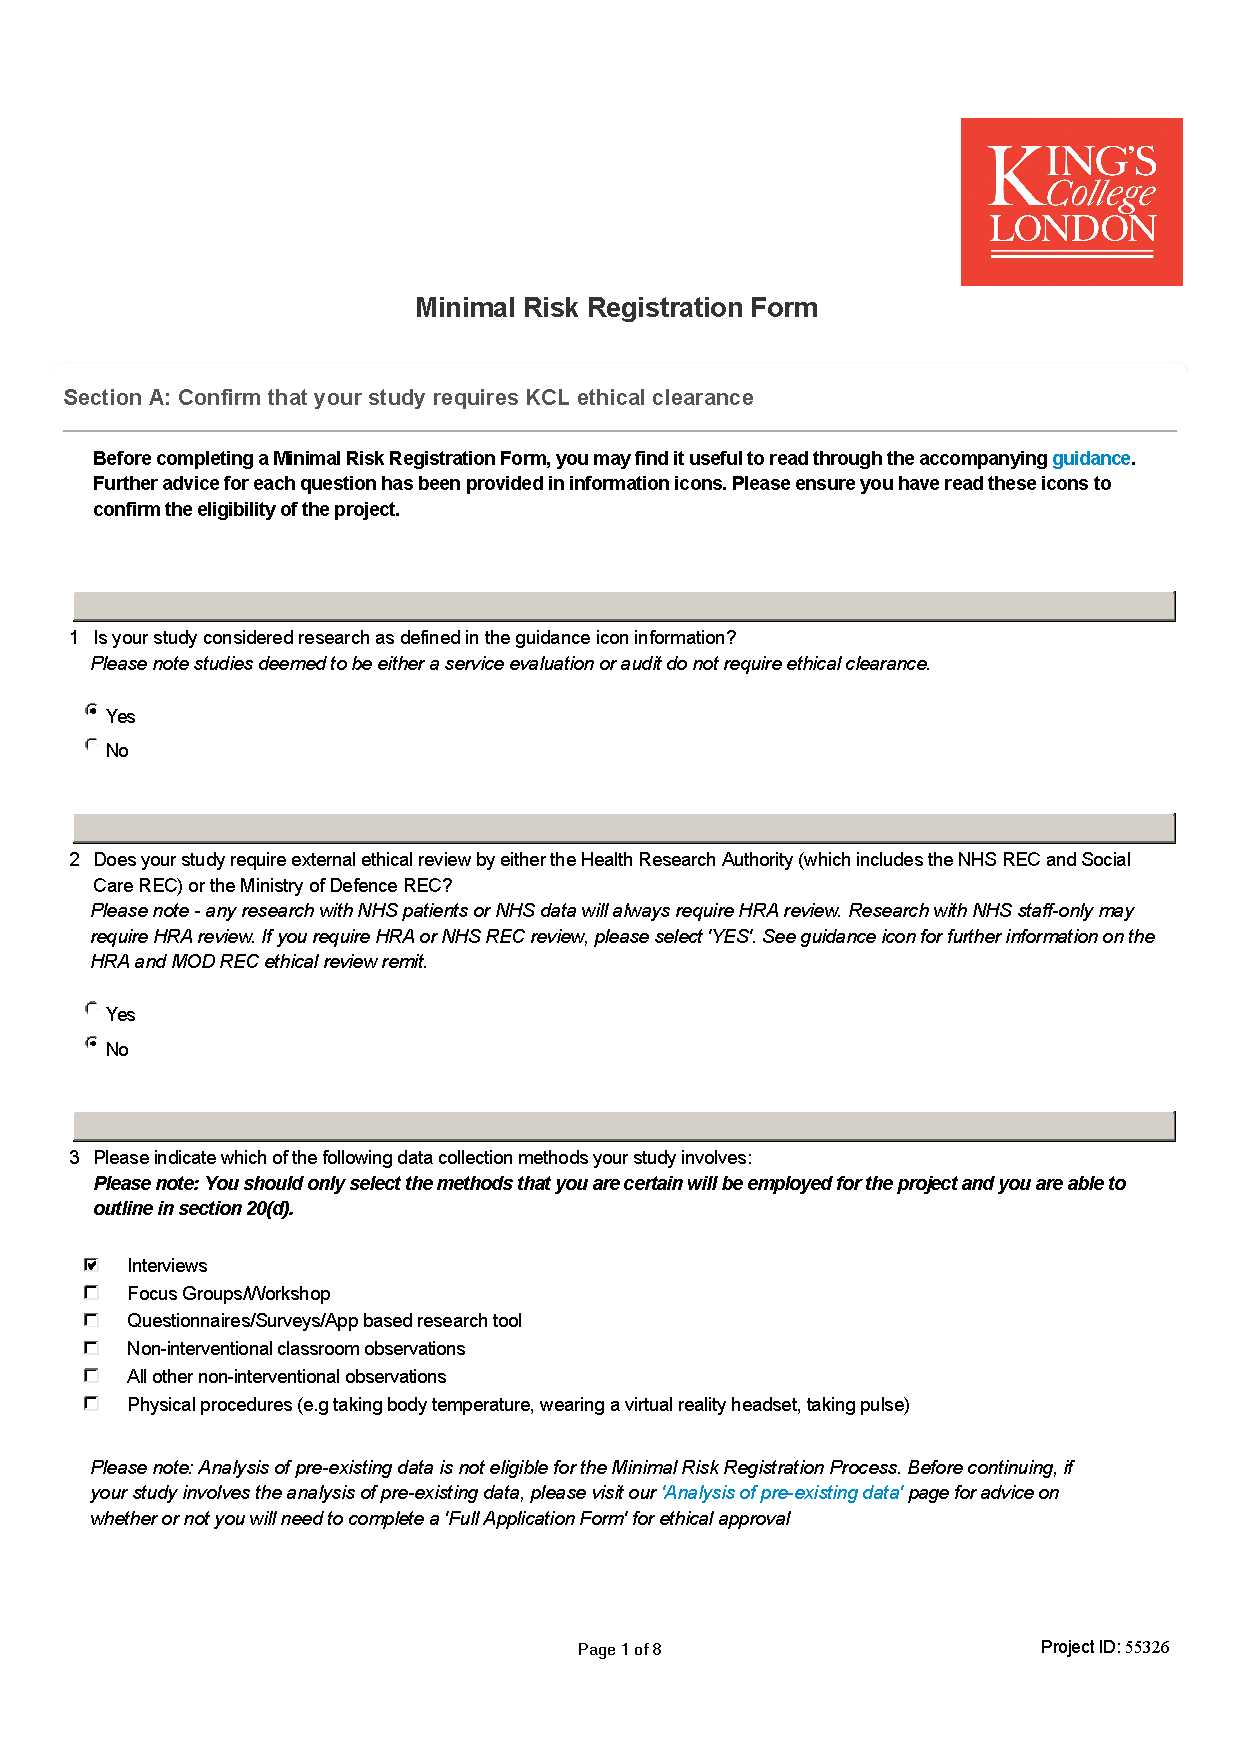
\includepdf[pages=-,pagecommand={\thispagestyle{plain}}]{appendix-materials/ethics/ethics-approval.pdf}%
}{%
  \noindent\textit{The file \texttt{appendix-materials/ethics/ethics-approval.pdf} was not found. Add it to the project (same path as on your local machine) and recompile the appendices document so this page shows the scanned approval.}%
}

\chapter{Source Code}
\label{app:source-code}

\section*{Authorship statement}

\noindent
I verify that I am the sole author of the programs contained in this folder, except where explicitly stated to the contrary.

\vspace{1em}
\noindent
\textbf{Signed:} Mert Ayranci \hfill \textbf{Date:} \today

\section{Submission contents}
\label{sec:source-submission}

\noindent
The complete source code is submitted alongside this report as a separate ZIP file. This appendix is intended as a navigation aid for that archive rather than a verbatim listing. It mirrors the structure of the prototype repository and gives a one-line description of every file or unit.

The prototype is a Next.js (App~Router) front-end written in TypeScript, styled with Tailwind CSS, and tested with Vitest and React Testing Library. Build and run instructions are provided in Appendix~\ref{app:user-guide}; the architectural narrative is given in Chapter~\ref{sec:components-state}.

\section{Repository layout}
\label{sec:source-layout}

\noindent
At the top level the archive is organised as follows:

\begin{center}
\small
\begin{tabular}{@{}P{3.6cm}P{9.8cm}@{}}
\hline
\textbf{Path} & \textbf{Purpose} \\
\hline
\texttt{src/app/} & Next.js App Router entry point, root layout, and global stylesheet. \\
\texttt{src/components/photo-\linebreak[0]revocation-demo/} & React components implementing every interface region of the prototype. \\
\texttt{src/lib/photo-\linebreak[0]revocation-demo/} & Domain types, helper functions, constants, and initial in-memory state. \\
\texttt{src/lib/} & Cross-cutting permission logic shared between components and tests. \\
\texttt{tests/} & Vitest suite organised into \texttt{unit/}, \texttt{components/}, \texttt{app/}, and shared \texttt{helpers/}. \\
Root configuration & TypeScript, Next.js, Vitest, ESLint, Tailwind PostCSS, and package manifest files. \\
\hline
\end{tabular}
\end{center}

\section{File index}
\label{sec:source-index}

\noindent
The following table lists every file in the submitted archive, grouped by directory, with a one-line description of its responsibility.

\subsection*{Application entry (\texttt{src/app/})}

\begin{center}
\small
\begin{tabular}{@{}P{4.6cm}P{9.0cm}@{}}
\hline
\textbf{File} & \textbf{Description} \\
\hline
\texttt{page.tsx} & Thin route component that mounts the \texttt{PhotoRevoca\-tionDemo} orchestrator on the root URL. \\
\texttt{layout.tsx} & Root layout, metadata, and font configuration applied to every page. \\
\texttt{globals.css} & Tailwind CSS entry point and global style resets. \\
\hline
\end{tabular}
\end{center}

\subsection*{Domain logic (\texttt{src/lib/})}

\begin{center}
\small
\begin{tabular}{@{}P{4.6cm}P{9.0cm}@{}}
\hline
\textbf{File} & \textbf{Description} \\
\hline
\texttt{photoModel.ts} & Pure permission model: \texttt{computeEffectiveStatus}, \texttt{forwardingAllowed}, \texttt{formatExpiryCountdown}, and time-limit helpers. \\
\texttt{photo-revoca\-tion-demo/types.ts} & TypeScript types for messages, permissions, participants, and modal state (single source of truth for the data model). \\
\texttt{photo-revoca\-tion-demo/constants.ts} & Static configuration: scroll-wheel sizing and the preset photo album. \\
\texttt{photo-revoca\-tion-demo/initialState.ts} & Default draft permissions, default time limits, initial conversation, and send-history seeds. \\
\texttt{photo-revoca\-tion-demo/helpers.ts} & Derivation helpers used by the UI: \texttt{getEffectivePermissions}, \texttt{getSourcePolicyPermissions}, view-once consumption checks, and download utilities. \\
\hline
\end{tabular}
\end{center}

\subsection*{React components (\texttt{src/components/photo-revocation-demo/})}

\begin{center}
\small
\begin{tabular}{@{}P{5.2cm}P{8.4cm}@{}}
\hline
\textbf{File} & \textbf{Description} \\
\hline
\texttt{PhotoRevocationDemo.tsx} & Central orchestrator: owns all shared state, handlers, and the four-handset layout. \\
\texttt{PhoneFrame.tsx} & Renders the device chrome for each stakeholder view and provides the per-handset overlay context. \\
\texttt{chatPanelPortalContext.tsx} & React context exposing portal and scroll references so overlays render inside the correct handset. \\
\texttt{MessageList.tsx} & Iterates a message array and dispatches each entry to a text or photo bubble. \\
\texttt{TextMessageBubble.tsx} & Renders text, reply previews, and accept/reject controls for access and revocation requests. \\
\texttt{PhotoMessageBubble.tsx} & Renders photo messages, the collapsible permission summary, role-aware action menu, and revocation submenu. \\
\texttt{PhotoPreview.tsx} & Renders a single photo asset with placeholder, view-once, and revoked variants. \\
\texttt{PhotoStackGrid.tsx} & Multi-photo collage layout for messages with several attached assets. \\
\texttt{PhotoStackLightbox.tsx} & Full-screen gallery viewer that portals into the active handset frame. \\
\texttt{ComposerView.tsx} & Pre-send composer with caption input, permission chips, and the screenshot warning. \\
\texttt{PickerSheet.tsx} & Photo picker sheet with multi-select and the dual \emph{Send}/\emph{Send with revocable permissions} actions. \\
\texttt{ScrollWheelColumn.tsx} & Reusable wheel control used by the time-limit picker. \\
\texttt{TimeLimitModal.tsx} & Post-send modal for adjusting a photo's expiry. \\
\texttt{RequestAccessPanel.tsx} & Inline footer panel for recipients to compose an access request. \\
\texttt{RequestRevocationPanel.tsx} & Inline footer panel for co-subjects to compose a revocation request. \\
\texttt{ViewOnceInChatModal.tsx} & Full-screen viewer that handles the view-once consumption lifecycle. \\
\texttt{ViewOnceSingleTick.tsx} & Small SVG indicator marking a view-once photo as consumed. \\
\texttt{PrototypeStateSummary.tsx} & Side panel exposing the live canonical permission record for evaluator inspection. \\
\hline
\end{tabular}
\end{center}

\subsection*{Tests (\texttt{tests/})}

\noindent
File names below are listed relative to the \texttt{tests/} root and are grouped by sub-directory.

\begin{center}
\footnotesize
\begin{tabular}{@{}P{5.8cm}P{8.0cm}@{}}
\hline
\textbf{File} & \textbf{Description} \\
\hline
\texttt{unit/photoModel.test.ts} & Unit tests for the pure permission model and time-limit helpers. \\
\texttt{unit/helpers.test.ts} & Unit tests for derivation helpers, including effective-status fallbacks. \\
\texttt{components/ComposerView.\linebreak[0]test.tsx} & Component tests for the caption input, permission chips, and the warning banner. \\
\texttt{components/PickerSheet.\linebreak[0]test.tsx} & Component tests for multi-select and the two send actions. \\
\texttt{components/PhotoMessageBubble.\linebreak[0]test.tsx} & Branch tests for active, revoked, view-once, and download-disabled variants. \\
\texttt{components/PhotoStackGrid.\linebreak[0]test.tsx} & Layout tests for multi-photo collages. \\
\texttt{components/PhotoStackLightbox.\linebreak[0]test.tsx} & Tests for the portalled full-screen gallery. \\
\texttt{components/RequestPanels.\linebreak[0]test.tsx} & Tests for both inline request panels (access and revocation). \\
\texttt{components/ScrollWheelColumn.\linebreak[0]test.tsx} & Tests for the duration picker primitive. \\
\texttt{components/TimeLimitModal.\linebreak[0]test.tsx} & Tests for applying and cancelling post-send expiry changes. \\
\texttt{components/TextMessageBubble.\linebreak[0]test.tsx} & Tests for replies and request response controls. \\
\texttt{components/ViewOnceInChatModal.\linebreak[0]test.tsx} & Tests for view-once open, close, and consumption state. \\
\texttt{components/ViewOnceSingleTick.\linebreak[0]test.tsx} & Snapshot test for the consumed indicator. \\
\texttt{components/PrototypeStateSummary.\linebreak[0]test.tsx} & Tests that the state panel reflects the canonical record. \\
\texttt{components/PhotoRevocationDemo.\linebreak[0]test.tsx} & Integration-style journeys covering revocation, forwarding, and request flows across handsets. \\
\texttt{app/page.test.tsx} & Smoke test that the route mounts the orchestrator without error. \\
\texttt{helpers/photoDemoUi.tsx} & Shared Testing Library locators and assertions reused across integration tests. \\
\hline
\end{tabular}
\end{center}

\subsection*{Documentation (\texttt{docs/})}

\begin{center}
\small
\begin{tabular}{@{}P{4.6cm}P{9.0cm}@{}}
\hline
\textbf{File} & \textbf{Description} \\
\hline
\texttt{README.md} (root) & Quick-start instructions, architectural overview, and test commands. \\
\hline
\end{tabular}
\end{center}

\subsection*{Configuration (root)}

\begin{center}
\small
\begin{tabular}{@{}P{4.6cm}P{9.0cm}@{}}
\hline
\textbf{File} & \textbf{Description} \\
\hline
\texttt{package.json} & Project manifest, dependency declarations, and \texttt{npm} scripts (\texttt{dev}, \texttt{build}, \texttt{start}, \texttt{test}, \texttt{test:coverage}, \texttt{lint}). \\
\texttt{package-lock.json} & Resolved dependency lockfile for reproducible installs. \\
\texttt{tsconfig.json} & TypeScript compiler configuration including the \texttt{@/*} path alias. \\
\texttt{next.config.ts} & Next.js framework configuration. \\
\texttt{next-env.d.ts} & Auto-generated Next.js TypeScript ambient declarations. \\
\texttt{vitest.config.ts} & Vitest configuration: jsdom environment, alias resolution, and coverage settings. \\
\texttt{vitest.setup.ts} & Test setup including \texttt{@testing-library/jest-dom} matchers. \\
\hline
\end{tabular}
\end{center}

\section{Notes}
\label{sec:source-notes}

\begin{itemize}
  \item All work on the prototype stopped once the archive was uploaded to KEATS. Several copies of the submitted version are retained locally and one of these copies will be used in the project examination.
  \item The deployed demonstration at \url{https://smart-photos.vercel.app} is built from the same submitted source and is provided only as a convenience; the canonical artefact for marking is the submitted ZIP archive.
  \item No third-party code is included in the archive beyond declared \texttt{npm} dependencies, which are installed at build time from \texttt{package.json} and \texttt{package-lock.json}.
\end{itemize}


\end{document}
